% !Mode:: "TeX:UTF-8:Main"
% arara: pdflatex
% arara: convert: {density: 160, otheroptions: -dispose previous -delay 20 -loop 1, format: gif}
% xarara: showfile: {format: gif}
\documentclass{article}
\usepackage[utf8]{inputenc} %probably not needed ...
\usepackage[T1]{fontenc}
\usepackage{geometry}
\geometry{papersize={128mm,96mm},margin=0.5cm} %\textwidth=11.8, \textheight=8.6
\usepackage[x11names,svgnames]{xcolor}
\usepackage{tikzducks}
\usetikzlibrary{shapes.geometric}
\usetikzlibrary{patterns,decorations.pathmorphing}
\pagestyle{empty}
\parindent=0pt
\usepackage{animate}
\usepackage{eso-pic}
\usepackage{xfp}
\newcommand\loopmax{10}
\definecolor{brazilgreen}{RGB}{0,168,89}
\definecolor{brazilyellow}{RGB}{255,204,41}%
\definecolor{brazilblue}{RGB}{62,64,149}%

\newcommand\tuglion{
     \begin{scope}[scale=0.5,xscale=-1,xshift=-1.3cm,yshift=-1cm,transform shape]
     \duck[body=brazilyellow,
     shorthair=brazilgreen]
     \path[preaction={fill, brazilblue},pattern=
     fivepointed stars, pattern color=white]
     \duckpathjacket;
     \fill[brown!50!black, rounded corners=1, rotate=-20] (0.8,0.75) rectangle (0.9,1.75);
     \fill[brown!50!black, rounded corners=1, rotate=-20] (0.4,1.7) rectangle (1.3,2.4);
     \fill[brazilgreen!40!black, rounded corners=1, rotate=-20] (0.45,1.75) rectangle (1.25,2.35);
     \node[rotate=-20, color=white] at (1.5,1.65) {\reflectbox{\footnotesize\bfseries 2018}};
     \end{scope}

     \begin{scope}[scale=0.4,xshift=5.3cm,yshift=-0.8cm,transform shape,]
     \duck[body=brazilyellow,
     shorthair=brazilgreen]
     \path[preaction={fill, brazilblue},pattern=
     fivepointed stars, pattern color=white]
     \duckpathjacket;
     \fill[brown!50!black, rounded corners=1, rotate=-20] (0.8,0.75) rectangle (0.9,1.75);
     \fill[brown!50!black, rounded corners=1, rotate=-20] (0.4,1.7) rectangle (1.3,2.4);
     \fill[brazilgreen!40!black, rounded corners=1, rotate=-20] (0.45,1.75) rectangle (1.25,2.35);
     \node[rotate=-20, color=white] at (1.5,1.65) {\footnotesize\bfseries TUG};
     \end{scope}
     }

\newcommand\duckpairsep{0.1cm}
\newcommand\duckleftscale{-1}
\newcommand\duckrightscale{1}
\newcommand\duckpair[1]{
\begin{scope}[#1]
  \begin{scope}[xshift=-\duckpairsep]
  \begin{scope}[xscale=\duckleftscale,transform shape]
  \duck[body=brazilyellow,
  shorthair=brazilgreen]
  \path[preaction={fill, brazilblue},pattern=
  fivepointed stars, pattern color=white]
  \duckpathjacket;

  \fill[brown!50!black, rounded corners=1, rotate=-20] (0.8,0.75) rectangle (0.9,1.75);
  \fill[brown!50!black, rounded corners=1, rotate=-20] (0.4,1.7) rectangle (1.3,2.4);
  \fill[brazilgreen!40!black, rounded corners=1, rotate=-20] (0.45,1.75) rectangle (1.25,2.35);
  \node[rotate=-20, color=white] at (1.5,1.65) {\scalebox{\duckleftscale}[1]{\small TUG}};
  \end{scope}
  \end{scope}

  \begin{scope}[xshift=\duckpairsep]
  \begin{scope}[xscale=\duckrightscale,transform shape]
  \duck[body=brazilyellow,
  shorthair=brazilgreen]
  \path[preaction={fill, brazilblue},pattern=
  fivepointed stars, pattern color=white]
  \duckpathjacket;

  \fill[brown!50!black, rounded corners=1, rotate=-20] (0.8,0.75) rectangle (0.9,1.75);
  \fill[brown!50!black, rounded corners=1, rotate=-20] (0.4,1.7) rectangle (1.3,2.4);
  \fill[brazilgreen!40!black, rounded corners=1, rotate=-20] (0.45,1.75) rectangle (1.25,2.35);
  \node[rotate=-20, color=white] at (1.5,1.65) {\scalebox{\duckrightscale}[1]{\small 2018}};
  \end{scope}
  \end{scope}
  \end{scope}
}

\begin{document}
\AddToShipoutPictureBG{%
 %\AtPageUpperLeft{%
 \begin{tikzpicture}[overlay,remember picture]
 \fill[Goldenrod1!50!white](current page.north west) rectangle (current page.south east);
 \fill[brazilgreen] (current page.north west) rectangle ([yshift=-2cm]current page.north east);
 \node [font=\LARGE\sffamily\bfseries,fill=brazilgreen,text=brazilyellow, inner ysep=7pt, anchor=north] (A)  at (current page.north) {Ordem e Progresso};
 \node[inner sep=7pt,minimum width=\paperwidth,fill=brazilblue,font=\Large\sffamily\bfseries,text=brazilyellow, anchor=north] at (A.south) {\begin{tabular}{cc}
 Come to the %39th Annual
 Meeting of the TeX Users Group\\
 July 20--22, 2018 -- Rio de Janeiro, Brazil
 \end{tabular}
 };
% %
  \pgfmathsetmacro\tmpaamplitude{2+0.01*mod(\csname c@page\endcsname,3)}%\show\tmpaamplitude
 \fill[brazilblue,decorate, decoration={snake,segment length={\tmpaamplitude cm}}]
  (current page.south west) circle [x radius=4.5cm, y radius=7cm, rotate=10];;

 \node[inner sep=0pt, anchor=south west] at (current page.south west){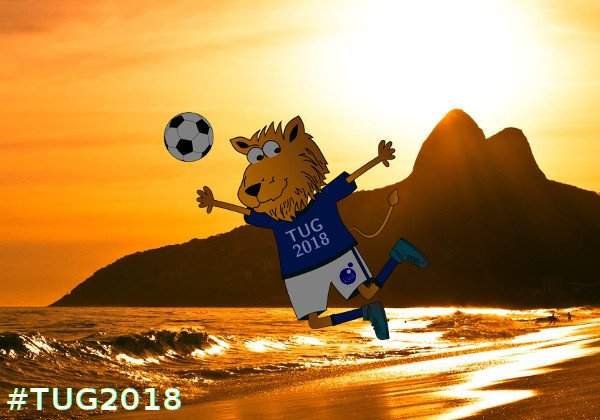
\includegraphics[trim=2cm 2cm 0cm 0cm,width=4cm]{tuglion}};

 \end{tikzpicture}
 }

%2.3 min
%3cm

\foreach\x in {0,1,2,3,4}
{\renewcommand\duckleftscale{1}%
\renewcommand\duckrightscale{-1}%
\renewcommand\duckpairsep{\fpeval{2.3+\x*0.2}cm}%
\begin{tikzpicture}
\path[use as bounding box] (0,0) rectangle (\textwidth,\textheight);
\tuglion

\duckpair{xshift=6.6cm,yshift=0cm}

\duckpair{xshift=4.7cm,yshift=3.7cm}

\duckpair{xshift=9.7cm,yshift=2.7cm}

\end{tikzpicture}\newpage
}

%0.8max: together
%0.1min:
\foreach\x in {0,1,2,3,4}
{%
\renewcommand\duckleftscale{-1}%
\renewcommand\duckrightscale{1}%
\renewcommand\duckpairsep{\fpeval{0.9-\x*0.2}cm}%
\begin{tikzpicture}
\path[use as bounding box] (0,0) rectangle (\textwidth,\textheight);
\tuglion

\duckpair{xshift=6.6cm,yshift=0cm}

\duckpair{xshift=4.7cm,yshift=3.7cm}

\duckpair{xshift=9.7cm,yshift=2.7cm}

\end{tikzpicture}\newpage
}
\end{document}
